\section{Experiments}
\label{sec:experiments}

Experiments are designed to cover different combinations of the framework's modules and to investigate the effectiveness of our approach. Specifically, each representation learner architecture is used for a variety of tasks, with the same policy module. 

\subsection{Tasks}
\label{sec:tasks}
% mention here the gym package?
Various tasks were explored as candidates to find the most suitable ones.

%   \begin{enumerate}
% 	\item Classic control tasks
% 	\item Simple pathing, obstacle pathing
% 	\item Dynamic scroller games (tunnel, evasion)
% \end{enumerate}

\paragraph{Classic Control Tasks} 
Conventional testing domains for RL agents include classic control tasks such as inverted pendulum, cart-pole, and mountain car.
Despite having similar physical properties like the sinusoidal nature of the tasks, these tasks have some interior aspects that make them less indicated for our goal. 
The primary issue is that the number of features used to describe the environments and the number of actions differ between tasks. For instance, cart-pole has two actions whereas mountain car has three. 
Furthermore, classic control tasks describe the different environments using a different number of features (e.g. four features in cart-pole while only two for mountain car).

To overcome the difference between number of actions and number of features in different tasks, homogeneous tasks were developed. They are therefore easily comparable to each other and do not require a mapping of the actions or visual input. 

\paragraph{Pathing Tasks}
We first propose a Pathing and Obstacle Pathing task, which are reasonably easy to solve and can be visualized - and learned - using a pixel representation of the state.
In these tasks, the agent needs to find a path from a starting point to an endpoint. 
In the Simple Pathing task there are no obstacles and the agent only needs to find the shortest path to the endpoint. 
In Obstacle Pathing there are obstacles that the agent needs to circumvent.

\paragraph{Scroller Games}
To test the framework on a wider transfer context, we also implemented four different scroller games:
Race, Evasion, Wall Evasion and Tunnel. The games share a single goal: reach the furthest point possible without hitting black pixels. 
In Race and Evasion, the obstacles have the same size as the agent, but the direction of the scrolling is different (top-down in Race and right-left in Evasion). Wall Evasion and Tunnel are different versions of Evasion. 
On the one hand, Wall Evasion has larger obstacles resembling walls, which increases the difficulty for the agent to survive. 
On the other hand, Tunnel generates continuous obstacles, with only a few free spots safe to navigate, looking as if the agent is placed in a tunnel. 
The reason why we developed those different - but similar - tasks is that we expect an agent that is able to transfer knowledge, to generalize all these tasks as general scroller games and therefore be able to successfully re-use previous experiences and knowledge in tasks similar enough.

\begin{figure}[ht!]
	\centering
	\begin{subfigure}{0.24\columnwidth}
		\centering
		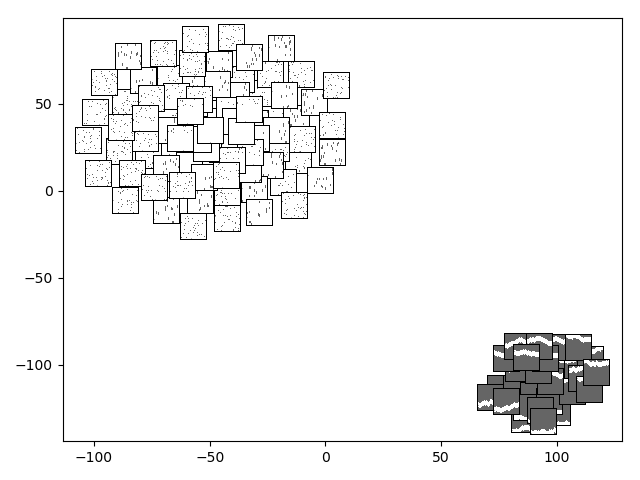
\includegraphics[width=\linewidth]{documentation/report/img/scroller_state.png}
		\caption{Race.}
		\label{subfig:race}
	\end{subfigure}%
	%
	\begin{subfigure}{0.24\columnwidth}
		\centering
		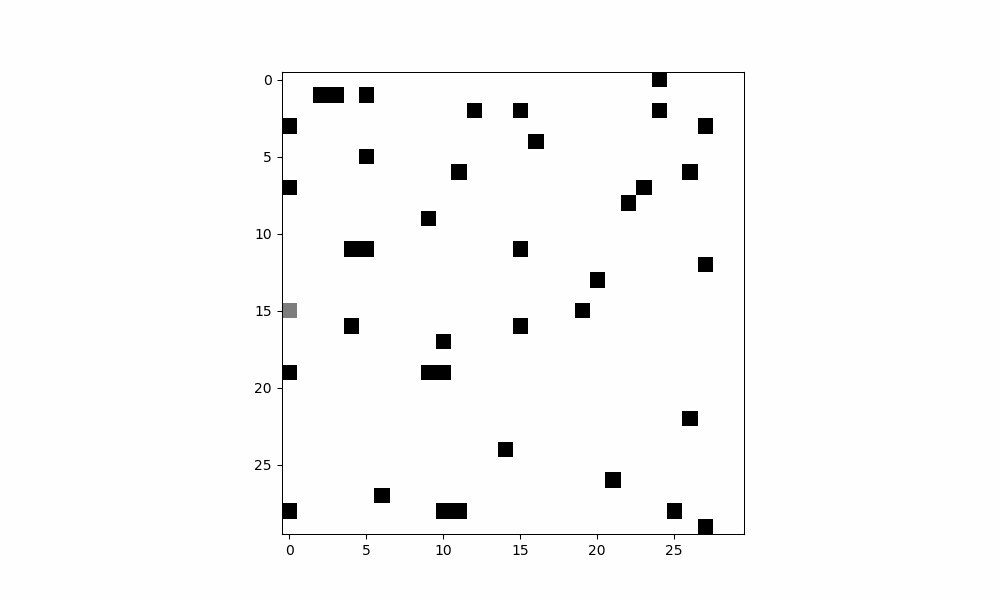
\includegraphics[width=\linewidth]{documentation/report/img/evasion.png}
		\caption{Evasion.}
		\label{subfig:evasion}
	\end{subfigure}
	%
	\centering
	\begin{subfigure}{0.24\columnwidth}
		\centering
		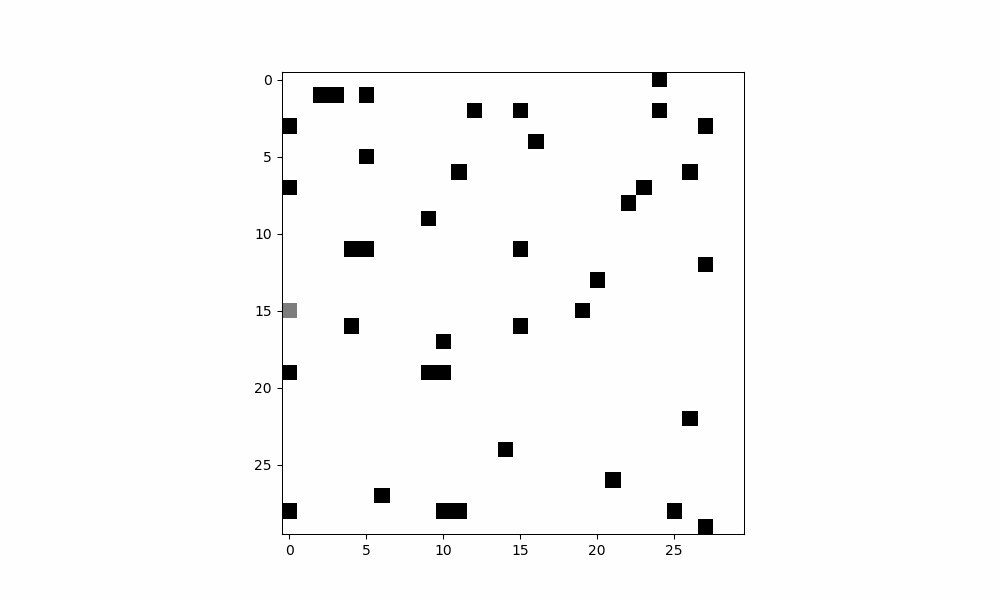
\includegraphics[width=\linewidth]{documentation/report/img/evasion.png}
		\caption{Walls \\ Evasion.}
		\label{subfig:wall_evasion}
	\end{subfigure}%
	% 
	\begin{subfigure}{0.24\columnwidth}
		\centering
		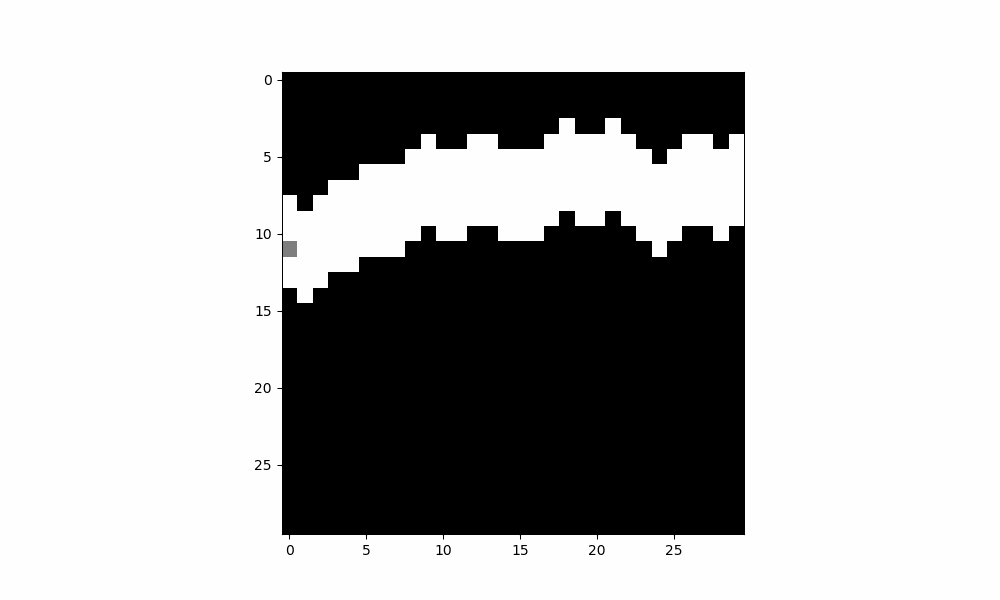
\includegraphics[width=\linewidth]{documentation/report/img/tunnel.png}
		\caption{Tunnel.\\}
		\label{subfig:tunnel}
	\end{subfigure}
	\caption{Visualizations of different Scroller games.}
	\label{fig:scrollers}
\end{figure}

\subsection{Experimental Setup}
In the following experiments, we evaluate our approach and determine which proposed representation module architecture is most suitable for transfer learning.

For all experiments the Double Deep-Q-Network is used as policy learner. We test the performance of the Convolutional Variational Autoencoder, the Janus architecture and the Cerberus architecture as representation modules.

\subsubsection{Experiments on Isolated Modules}
We first test the performance of the system's submodules in isolation to i) test their stand-alone performance and to ii) reason about their effects on the full model.

\paragraph{Representation Modules}
% what tasks, what representation modules
% motivate qualitative instead of quantitative analysis of results

The goal of the representation module is to embed the raw state into a latent representation that serves as a condensed input to the policy learner. The loss produced by the autoencoder architecture is expected to guide the latent space into a generalizable direction. To successfully leverage this representation, it needs to be able to reconstruct the input state well enough, even in a multi-task setting. That is, the latent space must contain enough information about the environment.

We obtain a comparison between current input and output of the architectures after 500,000 episodes of training. The comparison includes all the reconstructions that the network performs, therefore Janus is tested on current and next state and Cerberus on current state, next state and differences between current and next state. We will qualitatively analyze these comparisons, since a quantitative analysis on e.g. the losses is unsuitable due to the different demands made to the architectures, depending on the number of decoders. 

\paragraph{Policy Learner}
To test the performance of the policy learners in isolation, we still use the full model, but hold the representation module unchanged by its own loss.
That is, the weights of the autoencoder are not updated based on its decoder's reconstruction loss.
Due to the full backpropagation described in Section \ref{sec:approach}, the weights are still updated by the DDQN's loss, corresponding to the original architecture by \citet{DQN}. 

\subsubsection{Full System Experiments}
Once the modules are tested individually, we can test the framework in its entirety.
Each representation module paired with the policy learner is trained on the Tunnel task and on a set of Scroller tasks (Tunnel, Evasion, Walls Evasion) for multi-task learning. 
These subsets make it possible to test our approach by giving a previously unseen task to the trained network to investigate to which extent knowledge transfer is achievable.

Pathing tasks were not included in the final experiments for two main reasons: on the one hand, the agent needs a considerable amount of training time to reach the goal, especially in the first part of the training where its policy is purely random. On the other hand, Pathing tasks do not have any \textit{dynamics}, meaning that states differ only in the position of the agent. Since this difference is very small compared to the static obstacles and to the environment itself, it is difficult to represent the agent's position in the reconstruction of the representation learner.

To analyze how the transfer learning affects the training on a previously unseen task, two types of experiments were performed.

\textbf{Zero-shot} experiments, that measures how the system performs on a new task leveraging only the transferred knowledge, without any additional training.

\textbf{Learning improvement} experiments, that measure how the transferred knowledge affects the policy in a new training phase. 
For this type of experiment, the pre-trained network is further trained on the new task for $25,000$ episodes, and its performance is compared to the same architecture without any pre-training. 
It is worth to mention that in the second training phase, the loss of the representation learner is not back-propagated, so the whole system is updated only on the DDQN loss.

The parameters used in these experiments are listed in Table \ref{tab:hyperparas} and were chosen heuristically.

\begin{table}[t]
\centering
\begin{tabular}{@{}lll@{}}
\toprule
\textbf{Parameter} & \textbf{Value} \\ \midrule
number of episodes & $1,000,000$  \\
size of latent space & $32$  \\
memory delay & $10000$ steps  \\
initial epsilon & $1$  \\
initial epsilon with memory & $0.8$  \\
minimum epsilon & $0.01$  \\
epsilon decay & $3,000,000$  \\ \bottomrule
\end{tabular}
\caption{Table of hyperparameters used in the full system experiments. For the further training in the learning improvement experiment, $25,000$ episodes were used, with an epsilon decay of $300,000$, other parameters were not changed.  \label{tab:hyperparas}}
\end{table}
